\section{AI Assistant for Finding Destination}\label{section:ai-assistant}

\subsection{Problem Statement}
Users seeking their desired destinations are often overwhelmed by having to sift through extensive lists of rooms accompanied by lengthy descriptions. This process is time-consuming and inefficient, particularly when the user has only vague details about the destination and may not know the exact room code or name. In many cases, the user might recall only certain characteristics or features of a place rather than its specific identifier. Consequently, providing a simple static list of options fails to accommodate such nuances, leading to frustration and a suboptimal user experience. Therefore, there is a clear need for an intelligent system that simplifies this search process, enabling users to quickly and accurately locate their intended destinations.

\subsection{Solution}
To address these challenges and improve the efficiency of destination search, we integrate the capabilities of advanced LLMs into our application. In particular, we employ the \texttt{gpt-4o} model, which is well regarded for its proficiency in natural language understanding and generation. The system features an interactive chatbox where users can communicate directly with the LLM. Users can enter queries or descriptive phrases in their natural language, and the assistant responds with guidance, suggestions, or actions related to their requests.

Communication between the application and the LLM is facilitated via the OpenAI API. When a user sends a message, the application constructs an HTTP request that encapsulates it and sends it to the API server. The response is then processed and presented to the user. The request payload is structured as shown in the following code snippet:

\begin{lstlisting}[style=cSharp]
var requestBody = new RequestBody
{
    model = "gpt-4o",
    messages = new[]
    {
        new Message
        {
            role = "user",
            content = new[]
            {
                new Content
                {
                    type = "text",
                    text = message
                }
            }
        }
    },
    max_tokens = 300
};
new StringContent(JsonUtility.ToJson(requestBody), Encoding.UTF8, "application/json")
\end{lstlisting}

The \texttt{message} is not merely the user's raw input but a fully formatted message with appropriate prompting.

It is important to note that the \texttt{message} variable does not simply relay the raw input from the user; it is a carefully formatted string that incorporates a prompt designed to guide the LLM’s response effectively.

\hypertarget{prompt-engineering}{The art and science of crafting these prompts—commonly known as prompt engineering—is central to our solution. It involves designing the input so that the LLM produces accurate responses, is context-aware, and is directly aligned with the user's needs.} In our application, the prompt informs the model about the specific use cases and operational context of the assistant and instructs it to guide users toward providing the necessary details to facilitate accurate destination identification. The prompt used in our system is structured as follows:

\begin{lstlisting}[style=cSharp]
string prompt = @"
    Read this message from the user, process three cases:
        1. If the user asks for or describes a place, return a message instructing them to wait while the search and navigation are being processed. In addition, the message MUST start with an extra line containing the exact string \"PROCESSING\".
        2. If the user asks about the application's usage, return a message answering them based on the following description of the application: $application_description, and also introduce and guide them to use case 1 above.
        3. Otherwise, return a message to communicate with them, and also introduce and guide them to use case 1 above.
        
        For all cases, return only the message as you communicate with them; NO OTHER WORDS (except for the first case which includes one extra line).

        The message from the user: $message
";
\end{lstlisting}

This prompt ensures that the user can communicate smoothly with our AI assistant while receiving valuable information. If users provide a place's description, the model will return a formatted answer so that we can recognize it and use the description to further locate the destination in our database, as described in Section~\ref{sec:DestinationDataManagement}.

\begin{figure}[ht]
  \centering
  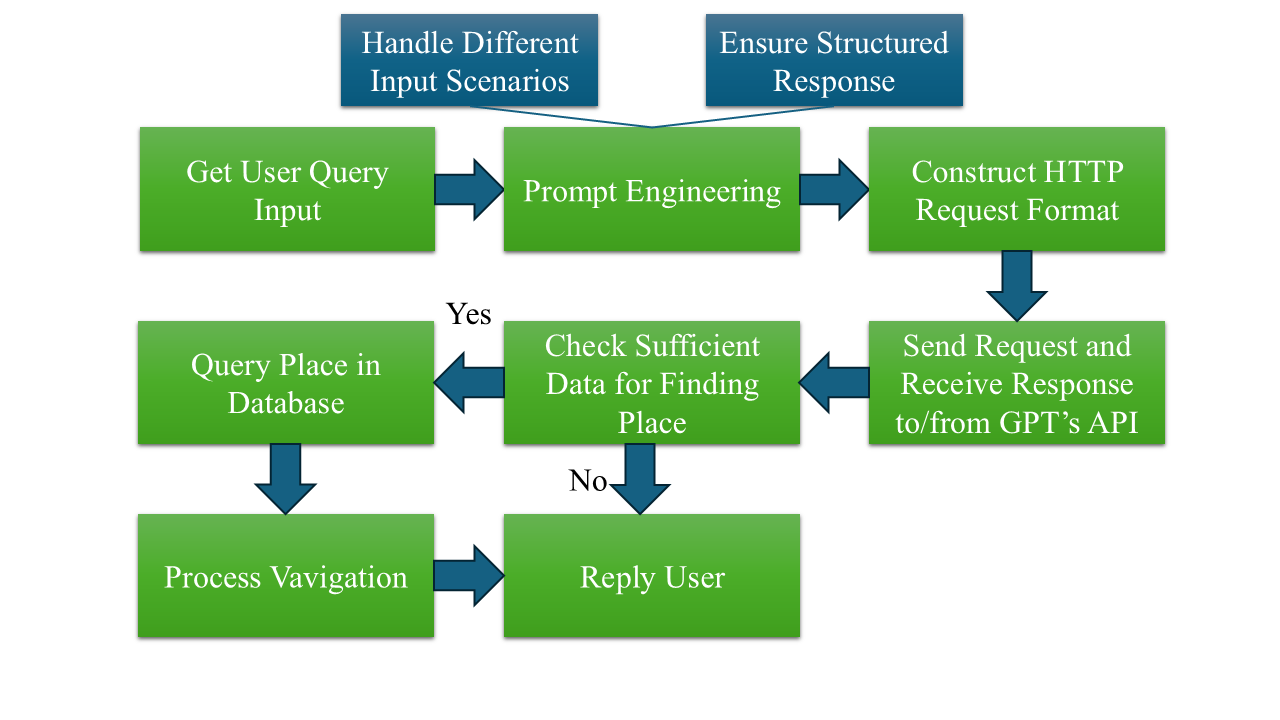
\includegraphics[scale=0.5]{content/resources/images/chap-problems-solutions/ai-assistant-0.PNG}
  \caption{Workflow of building AI Assistant}
  \label{fig:ai-assistant-0}
\end{figure}

